\chapter{The contributions}\label{sec:contributions}
Expectation-maximization is a very popular framework for different classification problems. It became extremly popular in segmentation of brain MRI during the last decade. However, it is not easy to understand the underlying theory.
\par
In this chapter, a very simple approach of the theory will be given.
\par
%Then, Kilian Pohl's contribution in slicer 3 and the problems encountered will be described.
\par
Finally, some solutions will be presented.
%present
Graphics files are inserted via the package \texttt{graphicx} which is
loaded in the document preamble (in file \texttt{report.tex}).
\par
Here we deal firstly with the inclusion of a single unlabelled diagram,
and then with captioned, labelled, and multiple diagrams.
\par
After that we consider tables of information.
%
\section{MRI Bias Field correction}
Here is a colour \texttt{.jpg} file, inserted in place without caption
and without a number for cross-reference. It's suitable only for a
simple self-explanatory diagram, used here and not again.

Bias correction is not efficient so we propose an other method, as part of the segmentation process.\\
Rescaling

\subsection{Interest}

Kilian algorithm is only accurate for small region bias correction, because au the gaussian model he uses.
Correction the bias in the whole volume first could enhance results.

\subsection{Our approach}

Gaussian distrib....
ITK filter
Automatic
\subsection{Results}
corrected not corrected
parameters explanation

\begin{center}
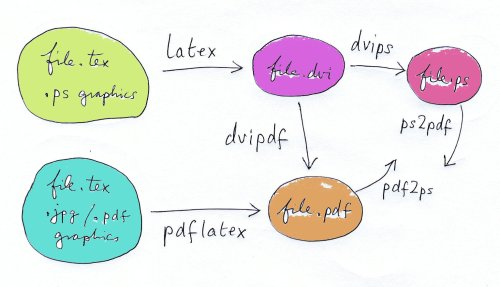
\includegraphics[width=.7\textwidth]{pic1.jpg}
%\includegraphics[width=.7\textwidth]{pic1new.jpg}
\end{center}
It shows the normal routes from a \LaTeX\ source (\texttt{.tex} file) to
\texttt{.ps} or \texttt{.pdf} output depending on the nature of the
graphics files included\footnote{An IDE such as TeXnicCenter has menu
buttons for each part of each route.}. \textit{Confusion over these
routes is a frequent source of grief}.
\par
This template has diagrams and graphs in \texttt{.jpg}
format\footnote{File extensions must be \texttt{.jpg} and not
\texttt{.JPG} or \texttt{.jpeg}.} and so its source is compiled to a
\texttt{.pdf} file with the command or menu button \texttt{pdflatex}.
\par
Mathematical software such as \textsl{Maple} and \textsl{Matlab} can
produce either \texttt{.ps} or \texttt{.jpg} diagrams, while cameras and
scanners\footnote{The figure itself is hand-drawn and scanned.} usually
produce \texttt{.jpg}. If accurate detail is vital, \texttt{.ps} is
best.
\par
With care, you can mix some graphics formats within a document. For
instance, if you compile to \texttt{.pdf} then you can use an
arbitrary mix of \texttt{.jpg}, \texttt{.png} and \texttt{.pdf}
graphics, but not \texttt{.ps}. And a document to be compiled to
\texttt{.dvi}, including \texttt{.ps} graphics, can include other
formats too if they are explicitly given \Quote{bounding boxes}. But
it's relatively tricky and you're better-off converting everything to
one format.
\par
Note that you can't include \texttt{.bmp} or \texttt{.gif} files at
all, but conversion of graphics files --- from \texttt{.bmp} to
\texttt{.jpg} for example --- is easily done with software like
\textsl{PhotoShop} \cite{PS} or \textsl{ImageMagick} \cite{IM}.
\par
It's simplest to keep your image files in the same directory as your
\texttt{.tex} files. Otherwise you can explore the mysteries of
\verb+\graphicspath+ \cite[Sec.~10.2.5]{MG}. In any case, use only
forward slashes in a directory specification. Names of directories and
of graphics files \textit{must not} include spaces!
%
\section{Intensity Normalization}
\subsection{Interest}
usefull if you need to do a lot of segmentations
enhance the rescaling..?
\subsection{Our approach}
background/brain
\subsection{Our implementation}
show results... corrected image...

It's awkward to flow text round a picture, but it can be done with
packages such as \texttt{picinpar} or \texttt{wrapfig}, as \comp\
explains \cite[Sec.~6.4.1]{MG}.
\begin{center}
\begin{minipage}[c]{.45\textwidth}\centering
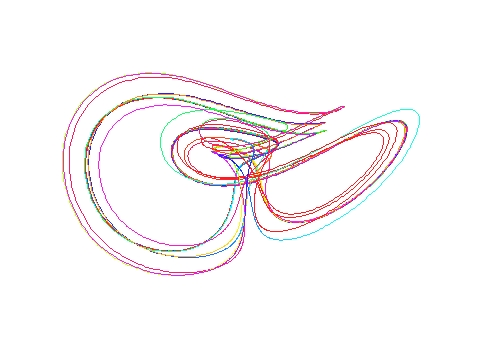
\includegraphics[width=.9\textwidth]{pic2.jpg}
\end{minipage}
\hfill\begin{minipage}[c]{.45\textwidth} And here's a \texttt{.jpg}
image side-by-side with some explanation, using the \texttt{minipage}
environment.\end{minipage}\end{center}
Something more elaborate sometimes gives unexpected results.
\par
\begin{figure}[ht]\centering
  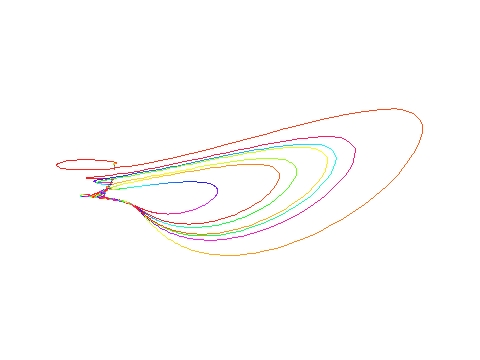
\includegraphics[width=.7\textwidth]{pic3.jpg}
  \caption{This is a caption explaining the diagram 
clearly and fully.}\label{fig:pic}
\end{figure}
That is, a picture \lq floating\rq\ in a \texttt{figure} environment
--- with a caption and number as in Fig.~\ref{fig:pic} --- might be
placed by \LaTeX\ on a page well after the text meant to accompany it.
\par
This happens if you have a relatively high density of graphics to
text. You may be able to deal with it by re-distributing the
pictures, changing the size of some of them, and the careful use of
paragraph breaks. Otherwise you may resort to \verb+\clearpage+,
which forces insertion of floating objects waiting to go in.
\par
The \nss\ book \cite{NSS} has Sec.~2.12 on the issue of \lq floating
bodies\rq\ and \comp\ has a whole chapter \cite[Chap.~6]{MG} on \lq
mastering floats'.
\par
Note that inside a \verb+figure+ (or \verb+table+) environment the 
\verb+\label+ must always {\em follow} the \verb+\caption+ --- see 
\cite[p.~67]{MG}.
\par
\begin{figure}[ht]\centering
\begin{minipage}[c]{.45\textwidth}\centering
  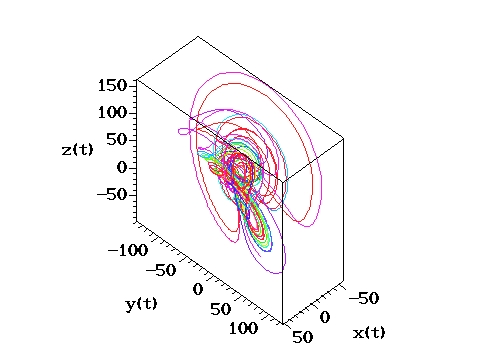
\includegraphics[width=.95\textwidth]{pic4.jpg}
  \caption{Caption to explain the diagram 
clearly and fully.}\label{fig:pictwo}
\end{minipage}\hfill
\begin{minipage}[c]{.45\textwidth}\centering
  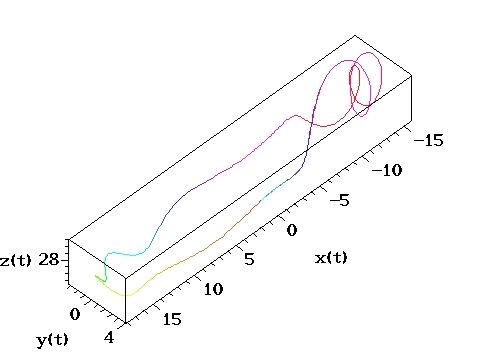
\includegraphics[width=.95\textwidth]{pic5.jpg}\\
  \caption{Caption to explain the diagram
clearly and fully.}\label{fig:picthree}
\end{minipage}
\end{figure}
Fig~\ref{fig:pictwo} and Fig.~\ref{fig:picthree} are two pictures
floating side-by-side, each in a \texttt{minipage} and each with its
own caption and label. This can be an economical way to insert multiple
diagrams.
\par
But don't get carried away and cram too many pictures together.
Be aware of the size-reduction that's often necessary, and maintain
legibility by choosing large enough font and weight for symbols,
axis-labels and other text.
\par
Figure captions should give plenty of information, because readers will
first skim the Introduction and Conclusions --- and then look at the
pictures. If you want (really really want) to hook them, make sure that
every important figure plus its caption is as self-explanatory as
possible.
%
\section{Class Distribution selection}\label{sec:CDS}
%
During parameters initialization, the user has to define each class distribution. The current methods presents some troubles so we present here a new approach to estimate each class distribution.
%
\subsection{Interest}
%
So far, the user haf two choices to define each class distribution. He could enter manually the intensities mean value and variance for each class, for each volume to be processed. This way, the user can be very precise and accurate when he defines each class. But it is very hard for the user to found the good mean value and variance for each class for each volume. Morever, each time he wants to process a new volume, he will have to redefine mean values and variances. This is not convenient and it can takes a ot of time. The next approch consisted in defining a class model by manual sampling. For each class, the user clics in the related part of the volume. With this methos, the problem is that you compute your mean value and variance using a few samples. Then, your mean values and variances are not accurate. That's why we proposed a new approach using a label map, to estimate each class model.
%
\subsection{Method used}
%
Create a label map. colors we choose a the same as the one we defined for each class.
then run algorithm which will estimate the mean value and covariance values.
\par
%
Algorithm..?
%
\par
Explain each colors
\par
\begin{figure}\centering
\begin{minipage}[c]{.45\textwidth}\centering
  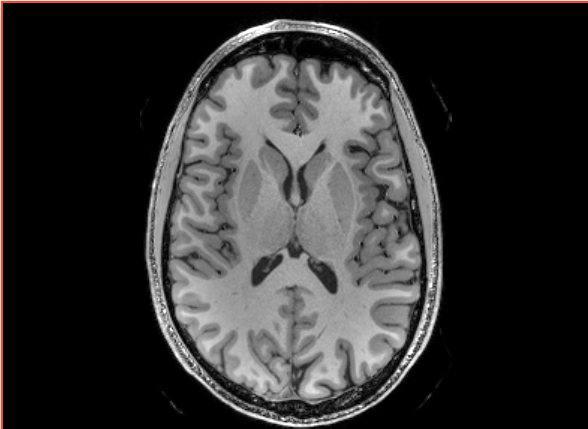
\includegraphics[width=.95\textwidth]{Images/Screenshots/T1ForLabel.png}
  \caption{Axial view of a T1 volume without the label map.}\label{fig:T1ForLabel}
\end{minipage}\hfill
\begin{minipage}[c]{.45\textwidth}\centering
  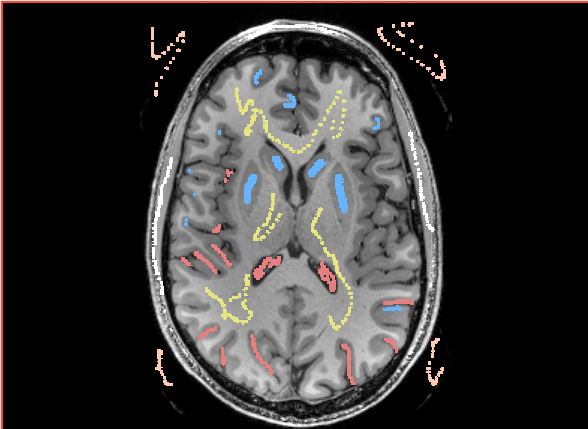
\includegraphics[width=.95\textwidth]{Images/Screenshots/LabelT1.png}
  \caption{Axial view of a T1 volume with the label map.}\label{fig:LabelT1}
\end{minipage}
\begin{minipage}[c]{.45\textwidth}\centering
  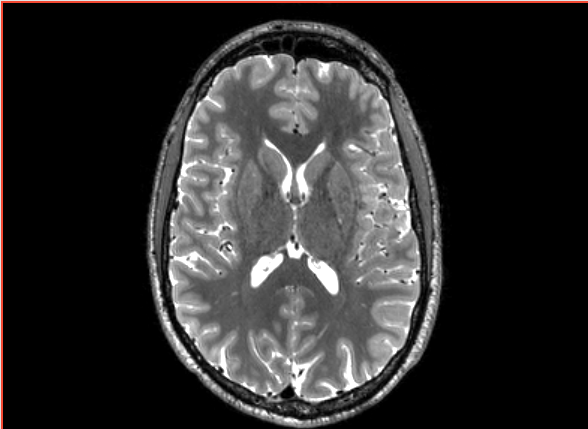
\includegraphics[width=.95\textwidth]{Images/Screenshots/T2ForLabel.png}
  \caption{Axial view of a T2 volume without the label map.}\label{fig:T2ForLabel}
\end{minipage}\hfill
\begin{minipage}[c]{.45\textwidth}\centering
  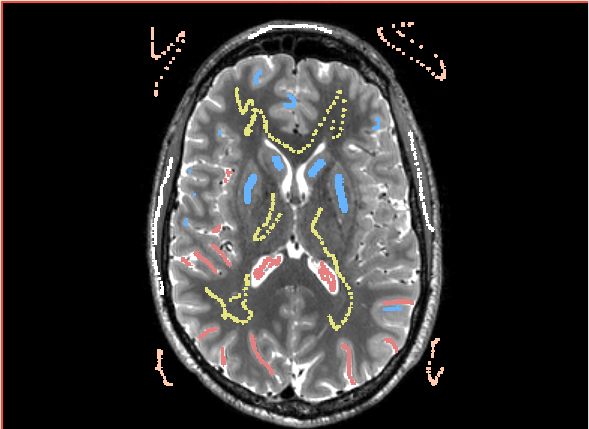
\includegraphics[width=.95\textwidth]{Images/Screenshots/LabelT2.png}
  \caption{Axial view of a T2 volume with the label map.}\label{fig:LabelT2}
\end{minipage}
\end{figure}
%
\section{Class Distribution visualization}\label{sec:tables}
%Besides figures you may want to include tables. Like figures, tables may
%be plain and simple --- short and for immediate and local use only ---
%and so put in place without a caption or label; or they may be
%complicated and important enough to need a reference label and an
%explanatory caption. Here are examples of each in turn.
An important contribution is a tool which allows to visualize the classes to be segmented distribution, through 2 volumes.
\subsection{Interest}
As we discussed in 
%partDFSD 
the EMS algorithm requires variance and mean values for each class to be segmented. So far, the user defines these parameters by selecting samples on the dataset.
%
exampleSDFSF
%
A main issue is that user user can know if the pixels he selected are really representative or not of the class he wants to select. Thus, our objective  was to find a way to give the user if his samples are reprenstative of not of a tissue.
\subsection{Method used}
%display a 3d image to alow the user to see the distribution
%\subsubsection{ used}
%compute variance and covariance matrix
\subsubsection{Problem's description}
Here is a brief description of the situation to let you understanding the problem. As input we have N images, K classes to segment, and for each class a mean value $\mu$, a variance $\sigma$ and covariance $\zeta$. The covariance is estimated for each couple of images. We will come back on it later.
%
where
%
Using these informations, we had to find a way to give the user usefull informations about the class distribution.
\subsubsection{Choices}
Our first idea was to display gaussian curves in 3D, for each class. The X and Y axes would be the intensity ranges for the to images we want to use.
The problem with this representation is that it does not contain any information about the number o
%
f pixels .  3d too sophisticated...?
%
To solve this problem, we decided to divide the problem in two parts.
The first part will consist in creating a "temperature map" as background.
The second part will consists in displaying ellipses over this map. This will give the user a good information about how good his selection was.
\subsubsection{Background creation}
First of all, the background has to be created. This background is a "temperature map".
We can present it as a two dimensions array. The height and the lenght of the array depend of the intensity range of the 2 volumes we want to process.
Then, we fill the array in an easy but useful way. Each 
%
case
%
of the array contains the number of occurence of an intensity pair at the same position, through the 2 volumes.

\begin{minipage}{1\textwidth}
%
\hrule
\textbf{\\Algorithm 1:} \textsc{BackgroundCreation}(V1,V2)
\hrule
%variables definition
\textbf{\\define}  RangeI1 $\leftarrow$  intensity range in V1\\ 
\textbf{define}  RangeI2 $\leftarrow$  intensity range in V2\\ 
\textbf{define}  A(RangeI1,RangeI2) $\leftarrow$ background\\  
%
\textbf{for each} pixel \textbf{i} in V1\\
\textbf{for each} pixel \textbf{j} in V2\\
%
$\triangleright$A(i,j)=A(i,j)+1\\
%
\textbf{return} A\\
%
\hrule
%
\end{minipage}

\subsubsection{Ellipse representation}
We will first start we a brief
%
rappel..
%
The covariance matrix is \\
Representing ellipse associated to this covariance matrix.\\
Maximum variance axe.Eigen values\\
Algorithm used.
Big and small axes of the ellipse\\
\subsection{Results}
show result
\par
First a simple table \dots\par
\begin{center}
 \begin{tabular}{|l||c|c|c|r|}
    \hline
    row 1& it's & just & as & easy \\ \hline
    row 2& as & this & \(E=mc^2\) & what \\ \hline
    row 3& could & be & simpler & ? \\ \hline
    row 4& as & easy & as & \(\Pi\) \\ \hline
  \end{tabular}
\end{center}
\par
Here it is again, now floating in a \texttt{table} environment, with
a caption and a label to identify it as Table~\ref{table:one}.
\begin{table}[h]
  \centering
\begin{tabular}{|l||c|c|c|r|}
    \hline
    row 1& it's & just & as & easy \\ \hline
    row 2& as & this & \(E=mc^2\) & what \\ \hline
    row 3& could & be & simpler & ? \\ \hline
    row 4& as & easy & as & \(\Pi\) \\ \hline
  \end{tabular}
  \caption{Floating table, with a caption to explain it 
clearly and fully.}\label{table:one}
\end{table}
The remarks about giving full information in figures and their
captions apply equally to tables, of course. So do the remarks about
unexpected placement of floating objects.
\par
If you need a long table, occupying more than a page, and which
can't reasonably be divided, then you need to delve into \comp\
\cite[Chap~5]{MG} to find the secret.
%---------
\section{Global Prior Estimation}

The last contribution to the EMS is a tool which provides the user an easy and fast way to estimate the global prior weights (GPW).(ref ch2 ...)

\subsection{Presentation of the problem}
This contribution is usefull in many different ways.
When you run the segmentation process,at the 6th step of the process, you have to provide to the algorithm an estimation of the GPW for each node in the tree. 
First of all if there are a lot of structures to segment, they user can spend a lot of time during this step. Indeed, for each part of this tree strcuture, they have to define the GPW. Moreover, the user may not know at all which weights to choose. This new approach will provide the users a good estimations of the weights to use. We must also keep in mind that the end users are physicists. They might don't understand what the parameters meanings and providing them a visual feedback could help them a lot.
\subsection{Our approach}
We divided the problem in two parts. The first part will be about providing the user a real-time feedback regarding the GPW estimation.
The second part will consist in developping an algorithm which fills automatically the tree.
\subsubsection{Fast user feedback}
We can divide the feedback part in 3 steps: the histogram computation and utilisation, the multicolumn list and the labelmap generated.
The histogram allows the user to manual segment classes based on intensity.
The multicolumn list allows the user to change the order of the classes in the histogram.
The labelmap provides to the user a visual feedback, base on the segmentation realized in the histogram.
Using these three complementary tools, the user, even if he is not initiated can estimate easily, accurately and rapidely the GWP.
\\schema
\subsubsection{Global priors evaluation}
The algorithm used to estimate the weight of each node is iterative. It starts from the root and goes to the leaves. It evaluates the weight of the childs of the active node at each iteration. Here is a description of the algorithms used to compute the GPW of each node.\\
DEscirption algo 1\\\\
%
%
\begin{minipage}{1\textwidth}
%
\hrule
\textbf{\\Algorithm 1:} \textsc{TreeWeightEstimation}(R, W)
\hrule
%variables definition
\textbf{\\define}  C = CHILD(R) $\leftarrow$ set of childrens of root R\\ 
\textbf{define}  LEAF(C)      $\leftarrow$ set of leaves of tree with roots C\\ 
\textbf{define}  H            $\leftarrow$ set of structure-specific information defined by LEAF(C) for each leaf\\
%
\textbf{update} W in childrens of root R with the results of \textsc{WeightEstimation}(C,LEAF(C),H)\\
%
\textbf{for each} node R' in CHILD(R) that is not a leaf\\
%
$\triangleright$\textsc{TreeWeightEstimation}(R', W)\\
\hrule
%
\end{minipage}
%
\\\\\\Descripton algo2\\
The algorithm used estimates the global prior of the leaves of the current node, based on the number of pixel which belong to the child classes.
This number of pixels is calculated from the segmentation computed in the histogram.(CF ..)\\\\
%
\begin{minipage}{1\textwidth}
%
\hrule
\textbf{\\Algorithm 2:} \textsc{WeightEstimation}(C,LEAF(C), W,H)
\hrule
%variables definition
\textbf{\\define}  T $\leftarrow$ set of total weight of leaves in LEAF(C). Leaves weights are contained in H\\ 
\textbf{define}  E      $\leftarrow$ set of weight for each node of C\\ 
\textbf{for each}  node of C\\
$\triangleright$E=E+H : Get the total weight of each node\\
%
W=E/T\\
%
\textbf{return} (W)\\
\hrule
%
\end{minipage}
%

\subsection{Results and discussion}
As we can see, the results obtained are good and accurate.The time of processing is fast and most of the people are now able to understand these parameters, even they are not familiar with EMS. This is an intuitive way to get an estimation of the GPW parameters.\\
Of course some sfsdfs must be done.
If there is a strong bias in the images we process, the pixels of a same class will have different values. Then, a segmentation based on intensity will provide bad results. Moreover, if the user wants to segment 2 classes which have the same color, just using the spatial information for example, they won't be able to use it properly.Thus, the user must always keep in mind that it is just an estimation and that he has to check if the values are accurate.

%Graphics files are evidently straightforward to include. If you need
%to go beyond the basics, then refer to \Quote{The Graphics Companion}
%\cite{GRM}.
%\par
%Tables are easy to use too, but don't misuse them. Lengthy data-sets can
%be supplied separately on CDrom. Put only summaries in the report,
%perhaps as an Appendix.
